\paragraph{curve-add}

\subparagraph{Target}
Implement the addition of two different curve points. this is a incomplete addition, you can refer to The halo2 Book \cite{website:halo2-book} to learn more about it.

\subparagraph{Constraints logic}
$(x_1,y_1) \ne (x_2,y_2)$, See \figref{fig:curve-add}.
\begin{figure}[!ht]
    \centering
    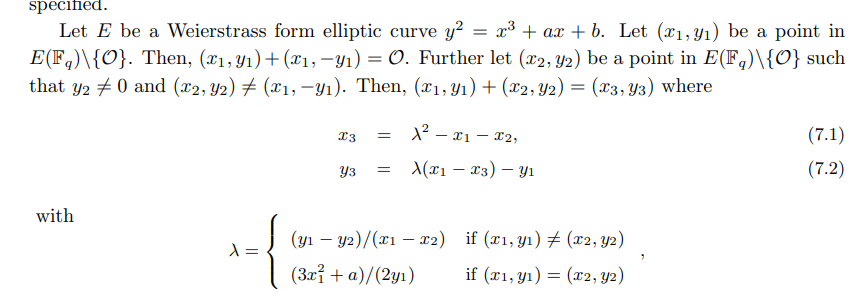
\includegraphics[width=0.8\textwidth]{curve-add.jpg}
    \caption{curve-add}
    \label{fig:curve-add}
\end{figure}

\subparagraph{Process layout}
See \figref{fig:curve-add-layout}
\begin{figure}[!ht]
    \centering
    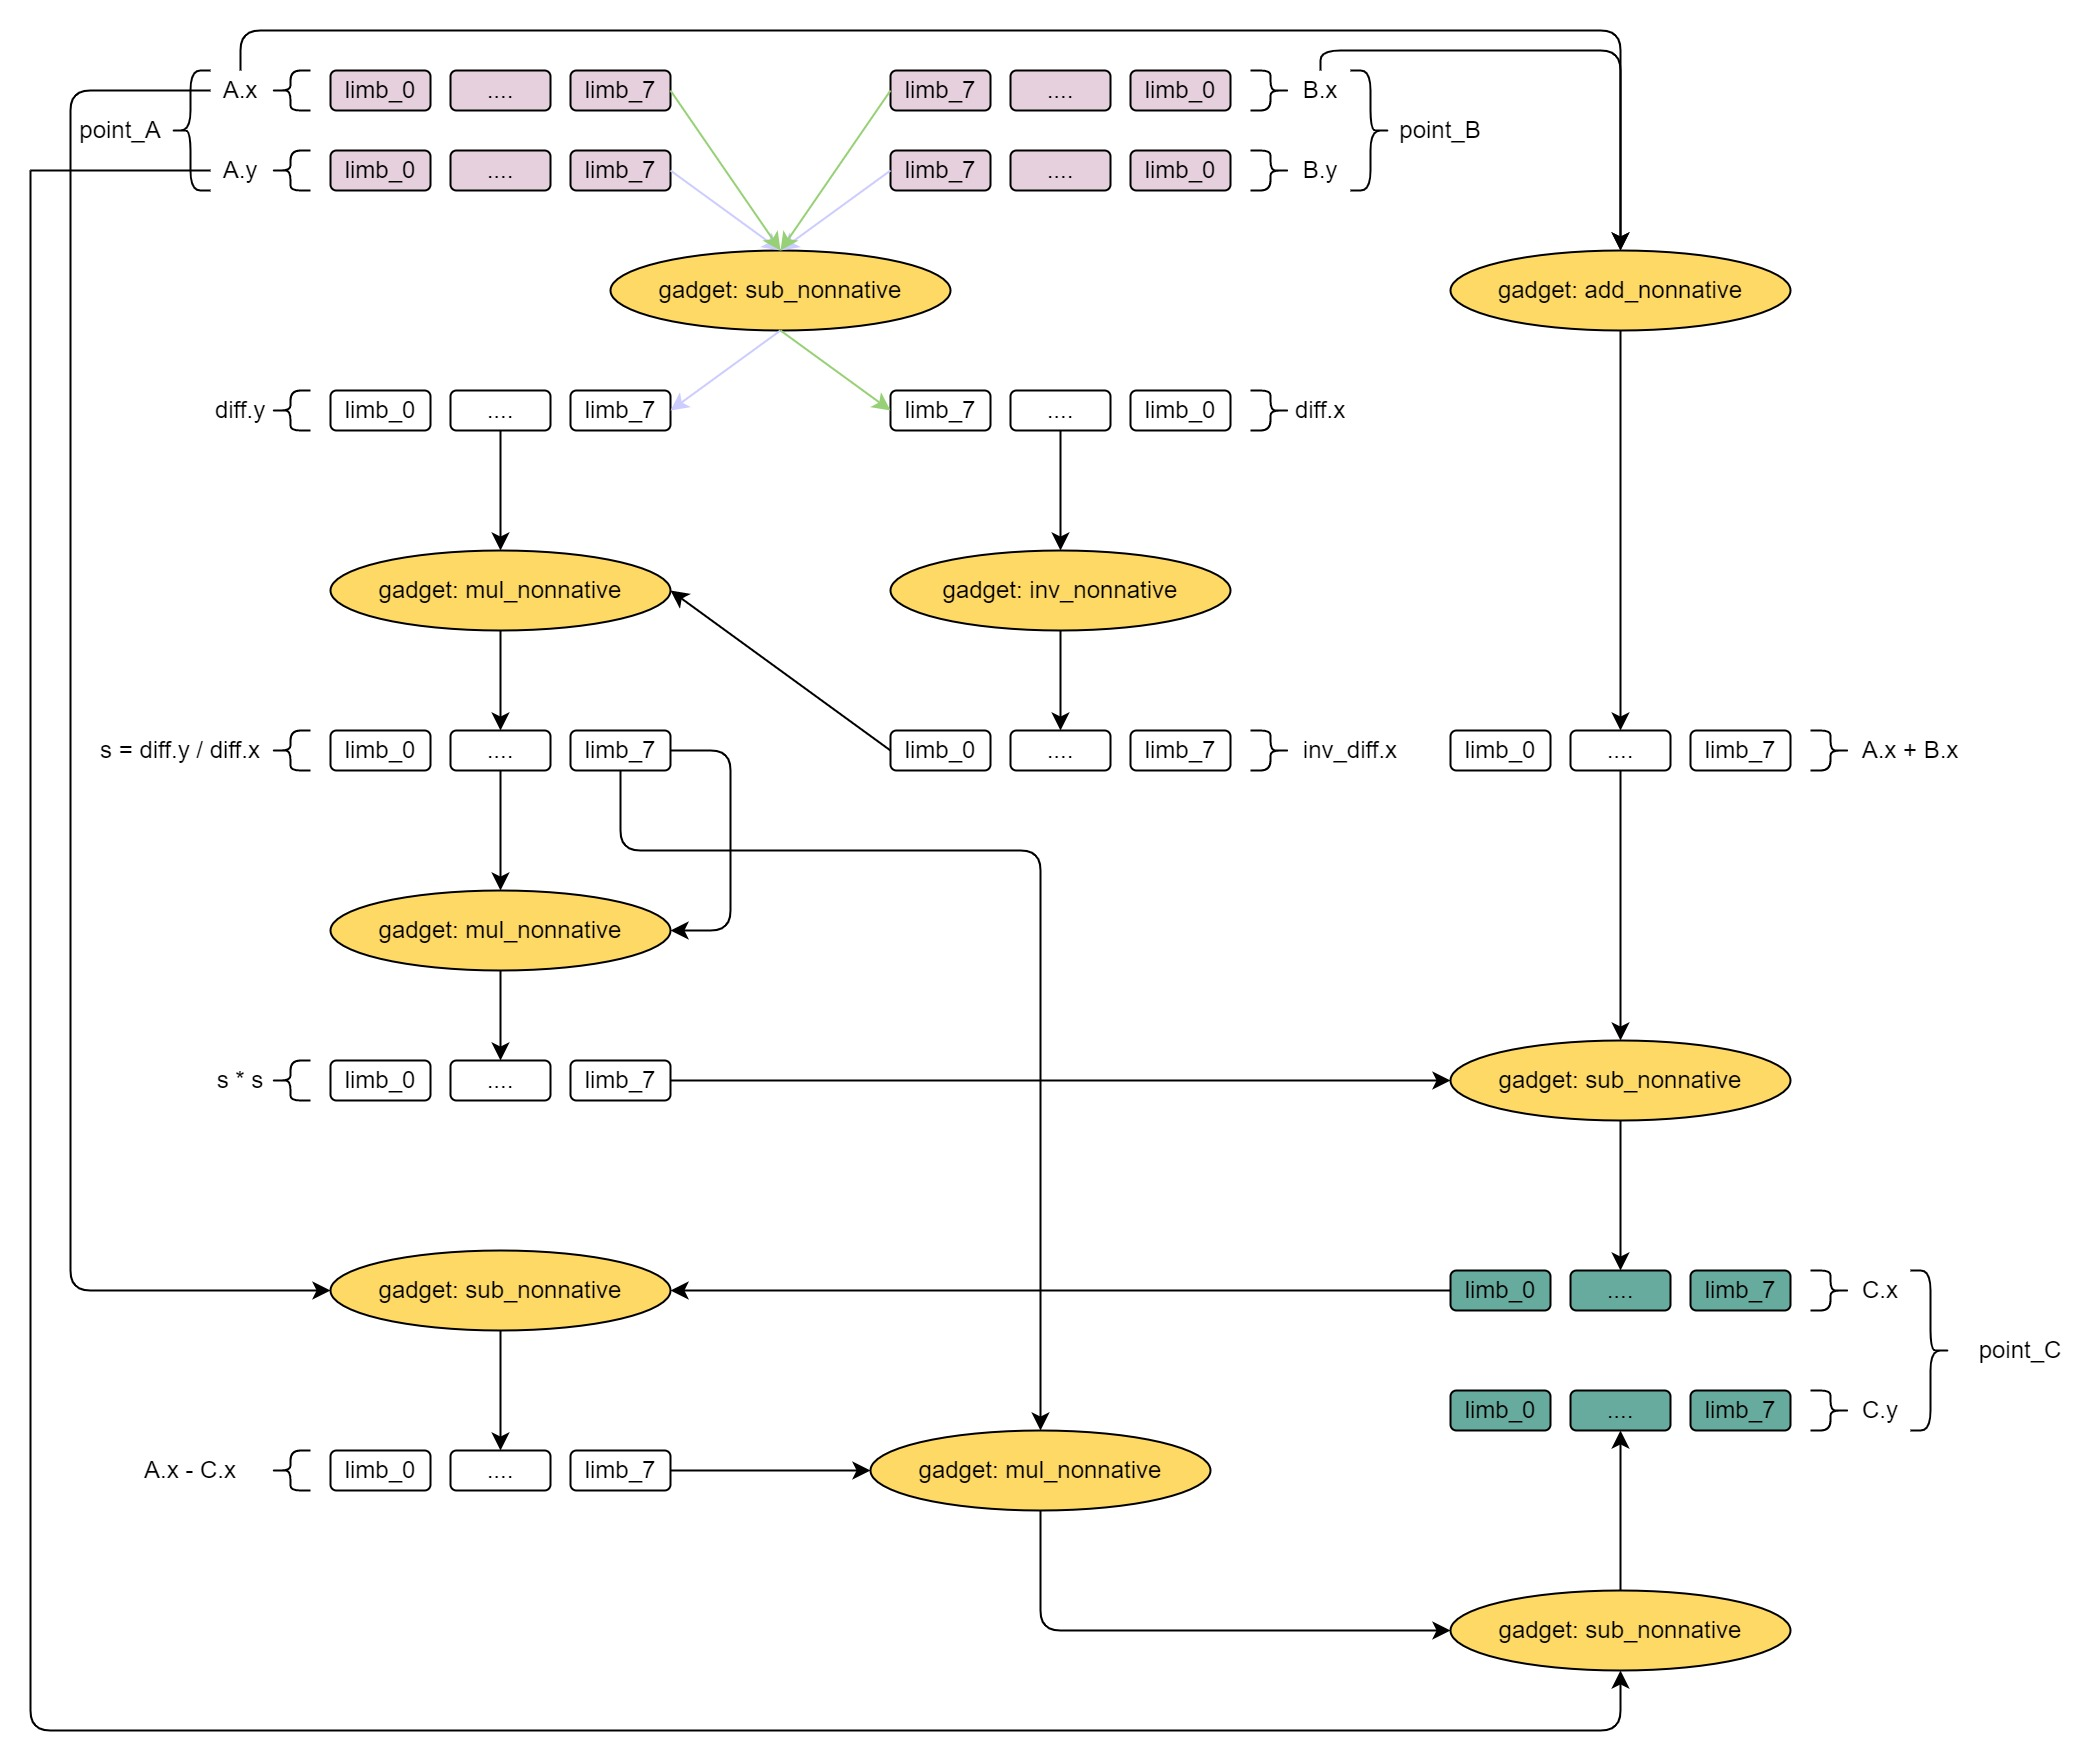
\includegraphics[width=0.8\textwidth]{curve-add-layout.jpg}
    \caption{curve-add layout}
    \label{fig:curve-add-layout}
\end{figure}

\subparagraph{Constraints info and costs}
\begin{itemize}
    \item gadget-sub-nonnative num: 5
    \item gadget-add-nonnative num: 1
    \item gadget-mul-nonnative num: 3
    \item gadget-inv-nonnative num: 1
    \item gate type num: 14
        \begin{itemize}
            \item 8: U32AddManyGate\{2,3,5,7,9,11,13,15\}
            \item 1: ComparisonGate
            \item 1: ArithmeticGate
            \item 1: U32ArithmeticGate
            \item 1: U32SubtractionGate
            \item 2: U32RangeCheckGate\{0,8\}
        \end{itemize}
\end{itemize}
